\documentclass[compress]{beamer}
%\documentclass[handout]{beamer}

\mode<presentation>
{
  \usetheme{CambridgeUS}      % or try Darmstadt, Madrid, Warsaw, ...
  \usecolortheme{default} % or try albatross, beaver, crane, ...
  \usefonttheme{default}  % or try serif, structurebold, ...
  \setbeamertemplate{navigation symbols}{}
  \mode<beamer>{\setbeamertemplate{blocks}[rounded][shadow=true]}
  \setbeamertemplate{caption}[numbered]
  \useoutertheme{infolines}
  \useoutertheme[subsection=false]{miniframes}
} 

\usepackage[english]{babel}
\usepackage[utf8x]{inputenc}
\usepackage{pifont}
\usepackage{amssymb}
\usepackage{xcolor}
\usepackage{tikz}
\newcommand{\xmark}{\ding{55}}%
\usepackage{eurosym}
\usepackage{graphicx}
\usepackage{comment}
% set colors
\definecolor{myNewColorA}{RGB}{0, 45,114}
\definecolor{myNewColorB}{RGB}{0, 45,114}
\definecolor{myNewColorC}{RGB}{0, 45,114} % {130,138,143}
\setbeamercolor*{palette primary}{bg=myNewColorC}
\setbeamercolor*{palette secondary}{bg=myNewColorB, fg = white}
\setbeamercolor*{palette tertiary}{bg=myNewColorA, fg = white}
\setbeamercolor*{titlelike}{fg=myNewColorA}
\setbeamercolor*{title}{bg=myNewColorA, fg = white}
\setbeamercolor*{item}{fg=myNewColorA}
\setbeamercolor*{caption name}{fg=myNewColorA}
\setbeamercolor{date in head/foot}{fg=white}
\setbeamercolor{page number in head/foot}{fg=white}


\titlegraphic{%
\vspace{0cm}
    
\includegraphics[width=4cm]{logo-vertical2.png}
}

\usepackage{subcaption}
% \usepackage{mathrsfs}

\usepackage{dirtytalk}
\usepackage{tcolorbox}
\usepackage{multicol}
\usepackage{multirow}
\usepackage{caption}
\usepackage{threeparttable}
\usepackage{pdfpages}
\usepackage{longtable}
\usepackage{adjustbox}
\usepackage{colortbl}
\usepackage{tikz}
\def\checkmark{\tikz\fill[scale=0.4](0,.35) -- (.25,0) -- (1,.7) -- (.25,.15) -- cycle;} 
\usepackage{pdfpages}

\usepackage{accents}
\newcommand{\ubar}[1]{\underaccent{\bar}{#1}}
%\usepackage{enumitem}

%% References - BEGIN
\usepackage[backend=bibtex8,style=authoryear-icomp,doi=false,url=false,isbn=false,eprint=false]{biblatex}
\renewbibmacro{in:}{}		% gets rid of the 'In' in front of the journal name
%\bibliographystyle{natbib}        
% \bibliography{references.bib}

% diagram (tree)
\usepackage{tikz}
\tikzset{
  treenode/.style = {shape=rectangle, rounded corners,
                     draw, align=center,
                     top color=white,
                     bottom color=blue!20},
  root/.style     = {treenode, font=\Large,
                     bottom color=red!30},
  env/.style      = {treenode, font=\ttfamily\normalsize},
  dummy/.style    = {circle,draw}
}

% Title page details: 
\title{Chapter 8: Taxes} 
\author{Jamie Hyder \\
    Discussion section 4}
\date{October 10, 2025}

\begin{document}

% Title page
\begin{frame}
    \titlepage 
\end{frame}

\begin{frame}{Outline}
    Today we will talk about:
    \begin{itemize}
        \item Taxes
        \begin{itemize}
            \item tax revenue
            \item social welfare
            \item tax incidence
        \end{itemize}
    \end{itemize}
\end{frame}


\begin{frame}{Taxes}
In the U.S. (Not necessarily in other countries!) direct price controls (ceilings/floors) are relatively rare.

\medskip

Taxes are much more common: \textbf{What is a tax?} \textbf{Who is a tax levied on?}

\medskip

\begin{block}{When taxes are levied we are concerned with:}
    The \textbf{Incidence of the tax}: how the burden of the tax is shared among participants (buyers \& sellers) in a market
\end{block}
\end{frame}

\begin{frame}{How do we determine tax incidence?}
    \begin{block}{Steps:}
        \begin{enumerate}
            \item Determine whether the tax is on buyers or sellers
            \item Decide which way the relevant curve shifts
            \item Examine how the shifts affect equilibrium price and quantity
            \begin{enumerate}
                \item Look at how buyers and sellers are affcected individually
            \end{enumerate}
        \end{enumerate}
    \end{block}
\end{frame}

\begin{frame}{Tax Revenue}
    How do we determine the tax revenue resulting from a tax?
    \begin{align*}
        \text{Tax Revenue } &= (P^{Buyer}_{Tax} - P^{Seller}_{Tax}) \times Q^*_{Tax} \\
        \text{Tax Revenue} &= \text{Tax Wedge} \times Q^*_{Tax}
    \end{align*}

    \begin{block}{How can we determine incidence from this equation?}
\begin{itemize}
    \item Burden on buyers: \((P^{Buyer}_{Tax} - P^*) \times Q^*_{Tax} \)
    \item Burden on sellers: \((P^* - P^{Seller}_{Tax}) \times Q^*_{Tax} \)
\end{itemize}
\end{block}
\end{frame}




\begin{frame}{Taxes}
    Let's return to the market for coffee...

    \begin{block}{Consider a $\$0.5$ tax on each cup of coffee \textit{levied on the sellers:}}
        \begin{itemize}
            \item Does this cause a shift in supply or demand?
            \item What will happen to $P^*$ or $Q^*$?
            \item What is the tax revenue/where is it on a graph?
            \item What portion falls on buyers and what portion falls on sellers?
        \end{itemize}
    \end{block}
\end{frame}

\begin{frame}{Taxes}
    In this example, buyers and sellers share the incidence of the tax.

\vspace{3mm}

    Really, it does not matter who the tax is levied on: 
    
    \[\textbf{tax on buyers = tax on sellers}\]

    \begin{block}{Let's consider the same questions under the following extreme cases:}
\begin{itemize}
    \item Demand is perfectly inelastic
    \item Supply is perfectly inelastic
\end{itemize}
    \end{block}
\end{frame}

\begin{frame}{Taxes \& Elasticity}
\begin{itemize}
    \item \textbf{Perfectly inelastic demand}: consumers buy the same amount of coffee no matter what $\implies$ consumers bear the entire incidence of the tax
    \item \textbf{Perfectly inelastic supply}: suppliers provide the same amount of coffee no matter what $\implies$ suppliers bear the entire incidence of the tax
\end{itemize}

\end{frame}


\begin{frame}{Taxes \& Elasticity}
   \begin{block}{ The relative elasticities determine the Tax Wedge: }
       This tells us which side of the market pays what portion of the tax.

       \medskip

       In general:
       \begin{itemize}
           \item Demand is more elastic than supply $\to$ \textit{suppliers} bear more of the burden
           \item Supply is more elastic than demand $\to$ \textit{buyers} bear more of the burden
       \end{itemize}
   \end{block}

   Really it is the \textbf{relative} elasticities which determine the wedge.
\end{frame}

\begin{frame}{Taxes \& Elasticity}
    \begin{block}{And... }
        The dead weight loss resulting from a tax depends on elasticity of supply and demand:
        \begin{itemize}
            \item Demand or supply is elastic $\implies$ large dead weight loss
            \item Demand or supply is inelastic $\implies$ small deadweight loss
        \end{itemize}
    \end{block}
\end{frame}

\begin{frame}{How do taxes and social welfare relate?}
    \begin{figure}
        \centering
        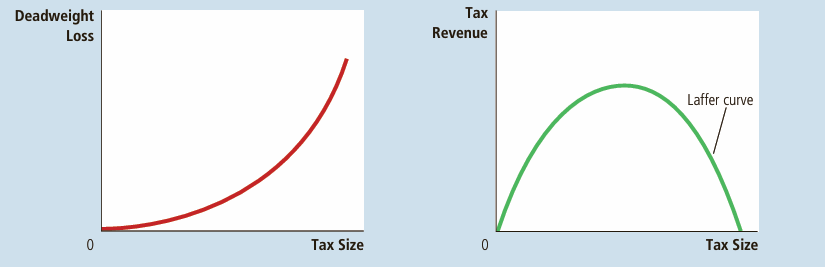
\includegraphics[width=0.95\linewidth]{laffer_dwl.png}
        \caption{Dead weight loss and tax revenue}
        \label{fig:placeholder}
    \end{figure}
\end{frame}

\end{document}